\subsection{Valgrind}
Valgrind was used for automatically detecting memory management bugs in the C executable. The command used was \code{valgrind --leak-check=full <command for parser>}.

It was used primarily to detect the number of allocations and freed blocks. For both applications it showed that more heaps were allocated than freed. Refer to section~\ref{buffer_overflow} for more information.

\begin{figure}[ht]
	\centering
	\begin{subfigure}{.5\textwidth}
		\centering
		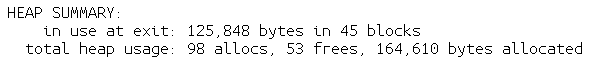
\includegraphics[width=.9\linewidth]{figures/valgrind_onlinebanking.png}
		\caption{Valgrind output for Online Banking}
	\end{subfigure}%
	\begin{subfigure}{.5\textwidth}
		\centering
		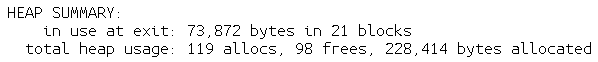
\includegraphics[width=.9\linewidth]{figures/valgrind_securebank.png}
		\caption{Valgrind output for SecureBank}
	\end{subfigure}
	\caption{Partial Valgrind output: heap management}
	\label{fig:cryptoshark}
\end{figure}